\chapter{Prezentacja warstwy użytkowej projektu}
\label{cha:wartstwa uzytkowa}

\section{Logowanie}

Po uruchomieniu aplikacji pojawia się okno ładowania, które szybko znika, a otwarty zostaje panel logowania, przedstawiony na \figurename~\ref{fig10}. Dostępne jest tutaj logowanie na konto, rejestracja nowego użytkownika,
a także logowanie jako gość, należy jednak pamiętać że gość ma jedynie dostęp do przeglądania oferty.
\begin{figure}[H]
    \centering
    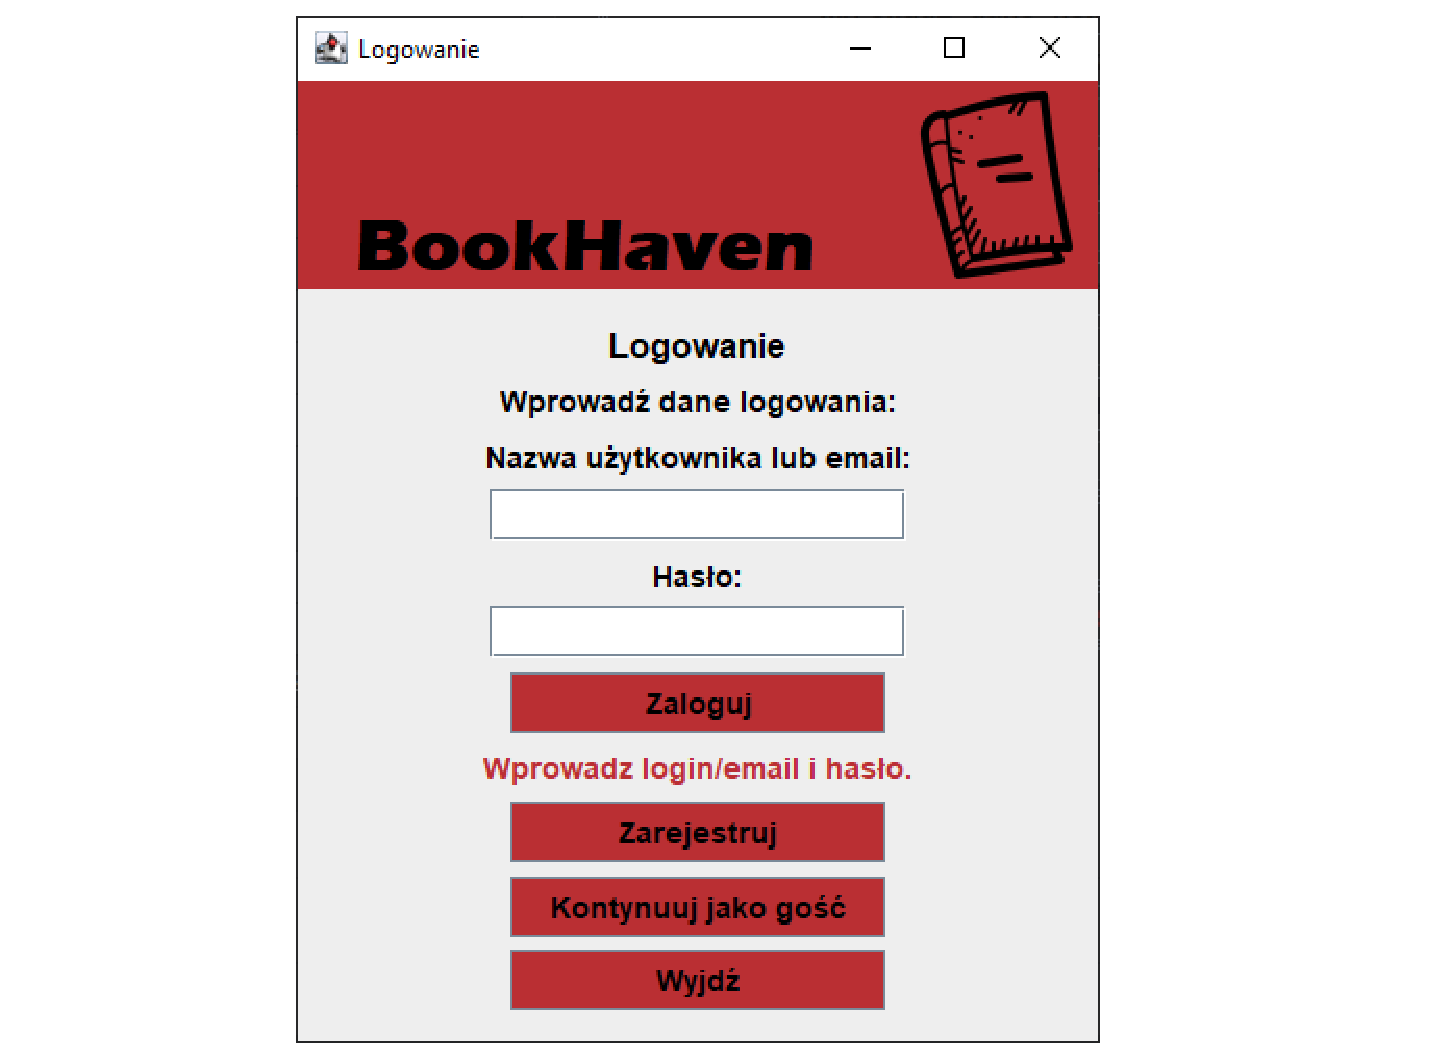
\includegraphics[width=\linewidth]{figures/fig_0010.eps}\\
    \caption{Panel logowania.\label{fig10}}
\end{figure}

\section{Panel klineta i gościa}

Po zalogowaniu na konto użytkownika otworzy się okno z sortowalnym i filtrowalnym katalogiem produktów dostpęnych w aplikacji. Zostało to przedstawione
na \figurename~\ref{fig12}. Dostępne są tutaj opcje zmiany ustawień konta (zmiana danych do późniejszej wysyłki), dodawanie produktów do koszyka, a także
wejście do koszyka, wraz z możliwością złożenia zamówienia przez klienta.
\begin{figure}[H]
    \centering
    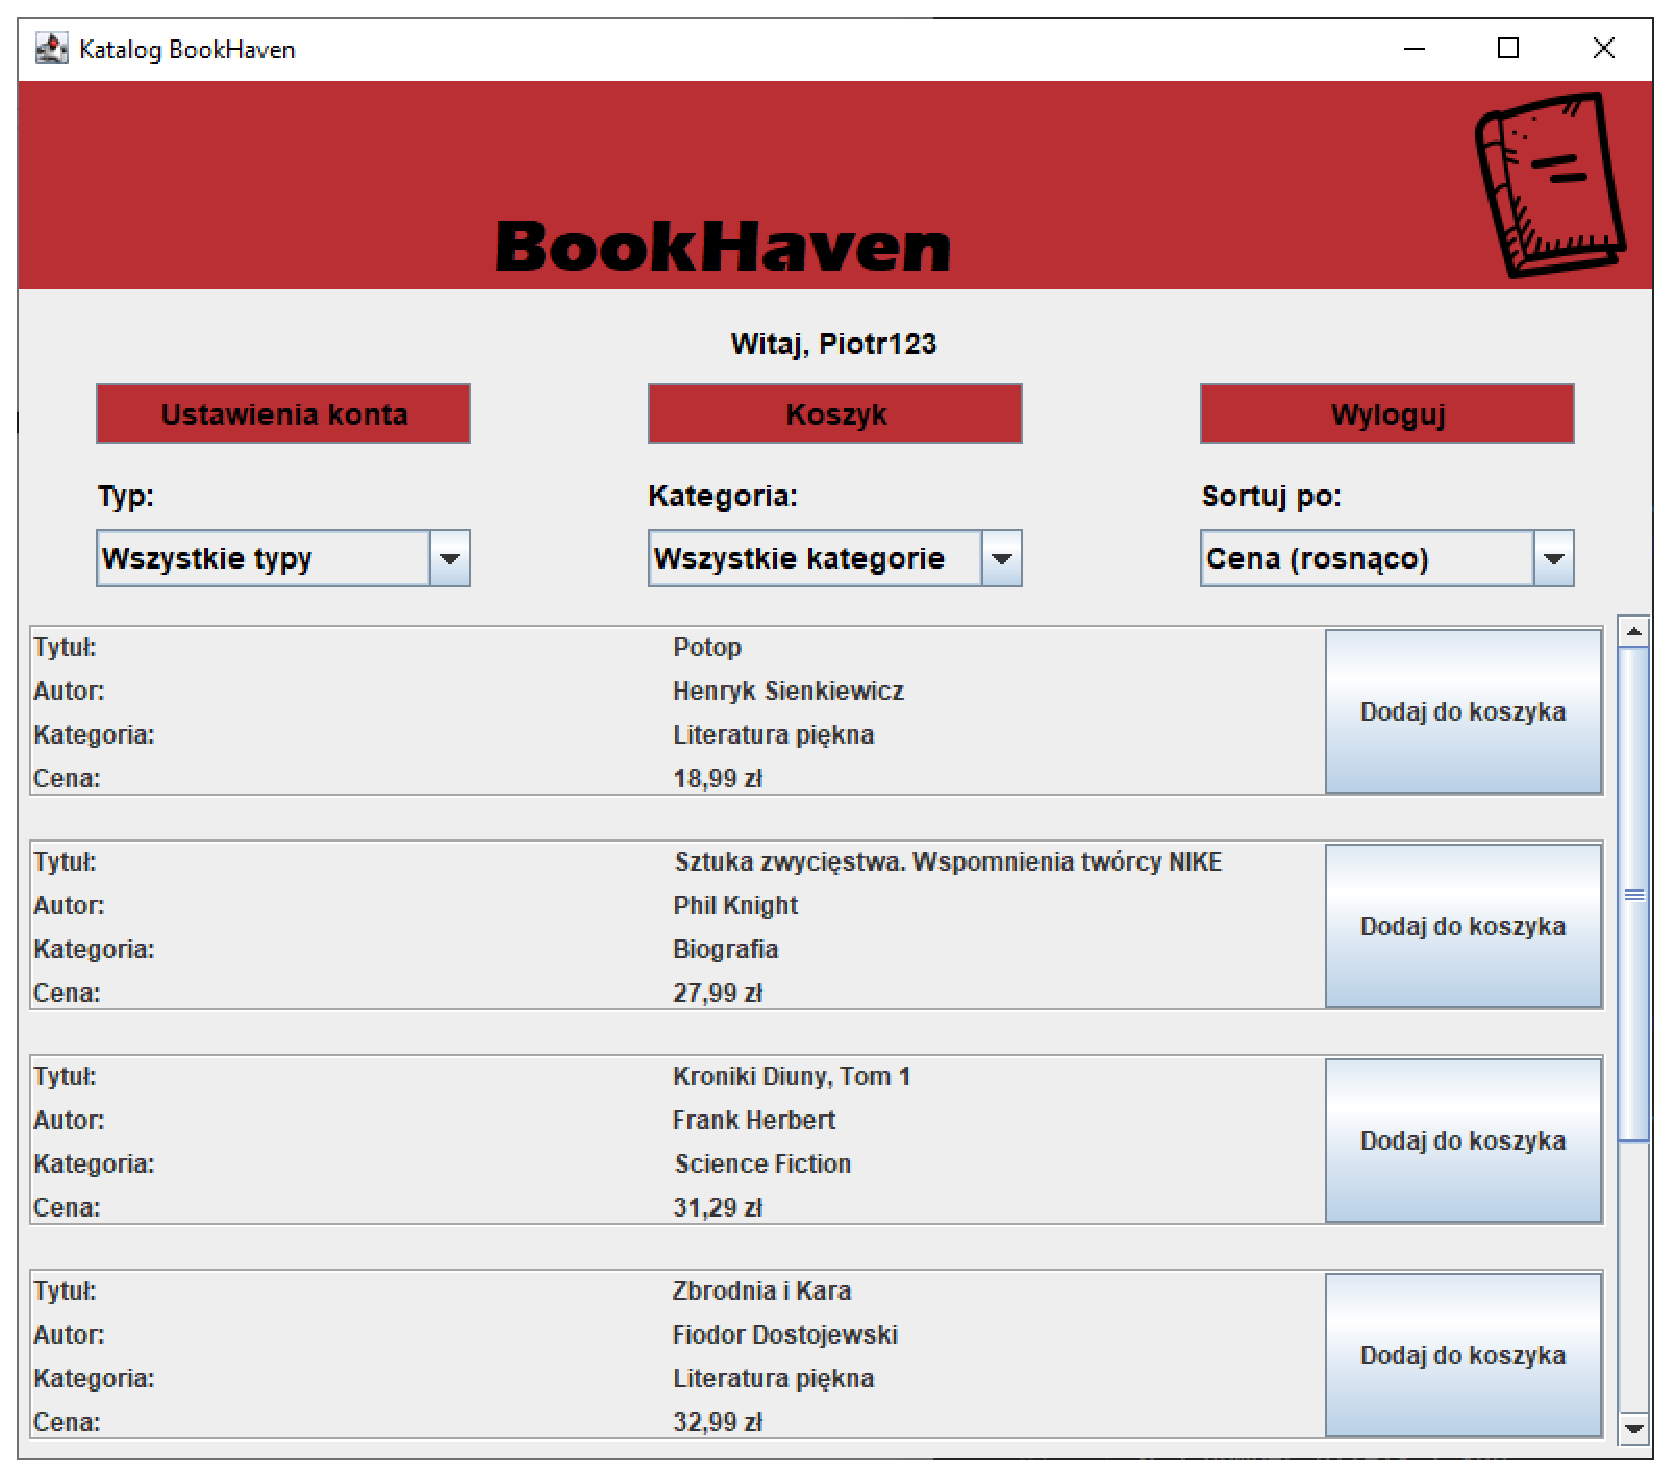
\includegraphics[width=\linewidth]{figures/fig_0012.eps}\\
    \caption{Panel klienta i gościa.\label{fig12}}
\end{figure}

\section{Panel administratora}

Po zalogowaniu na konto administratora (konto testowe o nazwie użytkownika "admin" oraz haśle "admin"), wyświetlony zostaje panel z możliwymi do podjęcia, przez niego, działaniami.
Panel ten przedstawiony jest na \figurename~\ref{fig11}. Administrator ma możliwość usuwania użytkowników z bazy, dodawania nowych administratorów oraz nowych produktów do bazy.
Zarządzanie produktami daje administratorowi narzędzia do usuwania i edycji istniejących produktów. Administrator może również zarządzać zamówieniami (przeglądać wszystkie zamówienia oraz zmieniać ich status).


\begin{figure}[H]
    \centering
    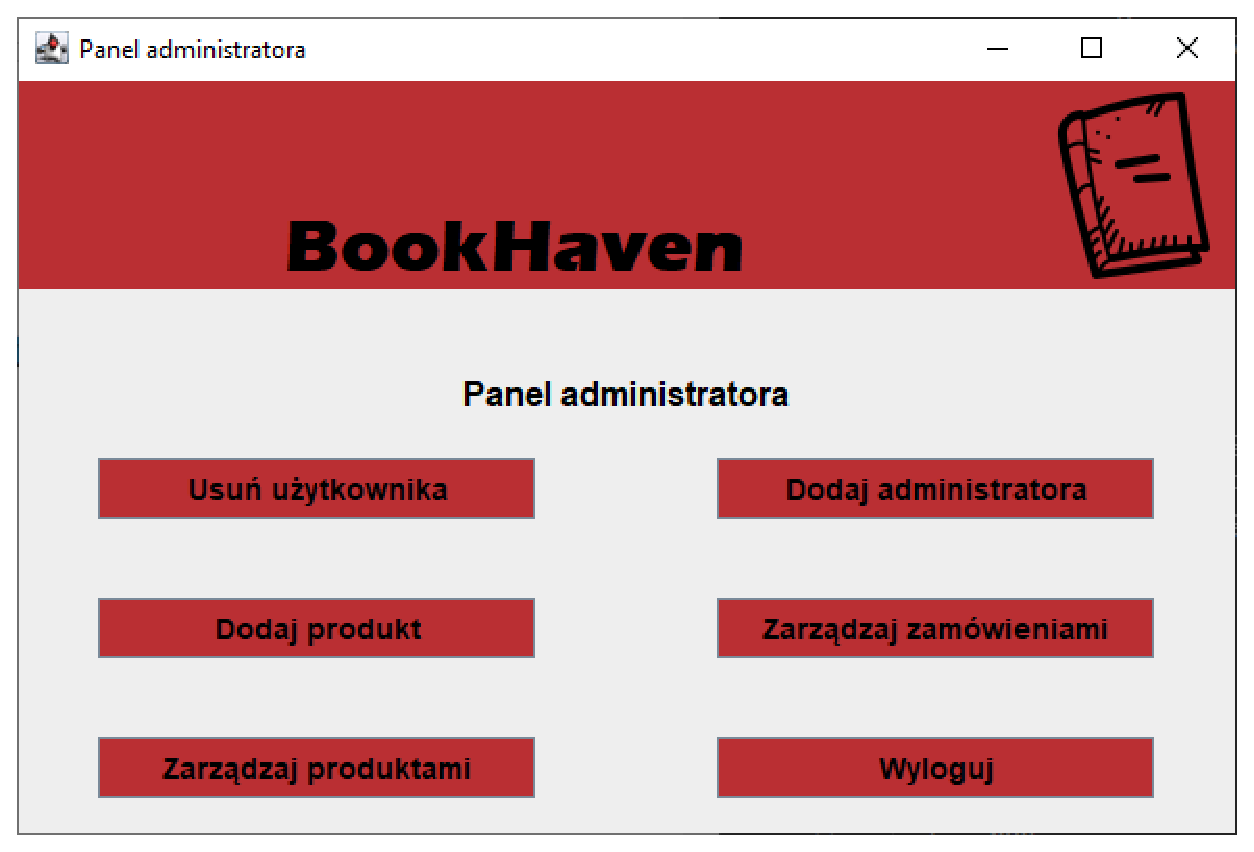
\includegraphics[width=\linewidth]{figures/fig_0011.eps}\\
    \caption{Panel administratora.\label{fig11}}
\end{figure}